\documentclass[11pt,a4paper]{article}

\usepackage[utf8]{inputenc}		% Configuro la codificación
\input{.command.tex}
% En el siguiente archivo se configuran las variables del trabajo práctico
%% \providecommand es similar a \newcommnad, salvo que el primero ante un 
%% conflicto en la compilación, es ignorado.

% Al comienzo de un TP se debe modificar los argumentos de los comandos


\providecommand{\myTitle}{TRABAJO PRÁCTICO Nº1}
\providecommand{\mySubtitle}{Recursividad}

\providecommand{\mySubject}{Algoritmos y Programación II (95.12)}
\providecommand{\myKeywords}{UBA, Ingeniería, C++, 95.12, Algoritmos y Programación}

% No es necesario modificar este
\providecommand{\myHeaderLogo}{header_fiuba}

\providecommand{\myAuthorSurname}{Lean Cole}
\providecommand{\myTimePeriod}{Año 2016 - 2\textsuperscript{do} Cuatrimestre}


% Crear los integrantes del TP con el comando \PutMember donde
%%		1) Apellido, Nombre
%%		2) Número de Padrón
%%		3) E-Mail (Si el mail contiene '_', escribirlos como '\_'
\providecommand{\CoverMembers}[0]
{		\PutMember{Lean Cole, Micaela} {96364} {mleancole@icloud.com} 
}

\providecommand{\myLstLanguage}{C++}

\Pagebreakfalse		% Setea si hay un salto de página en la carátula
\Indexfalse
\Siunitxfalse		% Si quiero utilizar el paquete, \siunixtrue. Si no \siunitxfalse
\Listingstrue		% Idem con paquete listings (programación)
\Keywordsfalse
				% Archivo con los comandos globales como Título y autores
%Preambulo para articulo científico de LaTeX

\usepackage[a4paper,left=3cm,right=3cm,bottom=3.5cm,top=3.5cm]{geometry} 	% Configuro la geometría del papel
%\usepackage{microtype}														% Mejora el "spacing" de las palabras
\usepackage[spanish]{babel} 												% Compatibilizo los signos del español
	\addto\captionsspanish{\renewcommand{\tablename}{Tabla}}				%% Redefino nombres preestablecidos por Babel
	\addto\captionsspanish{\renewcommand{\listtablename}{Índice de tablas}}	%% y así en vez de Cuadro dirá Tabla.
\usepackage{amsmath, amsfonts, amssymb}										% Entornos matemáticos, fuentes y símbolos
\usepackage{graphicx}														% Necesario para insertar figuras
\usepackage{fancyhdr}														% Para manipular headers y footers
\usepackage[usenames]{color}											% \color{color deseado} {lo que querés que tenga color}
\usepackage{subcaption}														% Permite captions del tipo 1a, 1b
\usepackage{multirow}														% Para tablas
\usepackage{float}

\ifListings
	\usepackage{listingsutf8}

	\definecolor{mygreen}{rgb}{0,0.6,0}
	\definecolor{mygray}{rgb}{0.5,0.5,0.5}
	\definecolor{mymauve}{rgb}{0.58,0,0.82}
	
	\providecommand{\lstinputpath}[1]{\lstset{inputpath=#1}}

	\lstset{
		backgroundcolor=\color{white},   % choose the background color; you must add \usepackage{color} or \usepackage{xcolor}
		inputencoding=utf8/latin1,
		basicstyle=\ttfamily\footnotesize,        % the size of the fonts that are used for the code
		breakatwhitespace=false,         % sets if automatic breaks should only happen at whitespace
		breaklines=true,                 %% sets automatic line breaking
		captionpos=t,                    %% sets the caption-position to top 
		commentstyle=\color{mygreen},    % comment style
		deletekeywords={...},            % if you want to delete keywords from the given language
		escapeinside={\%*}{*)},          % if you want to add LaTeX within your code
		extendedchars=true,              % lets you use non-ASCII characters; for 8-bits encodings only, does not work with UTF-8
		frame=single,	                 %% adds a frame around the code
		keepspaces=true,                 % keeps spaces in text, useful for keeping indentation of code (possibly needs columns=flexible)
		keywordstyle=\color{blue},       % keyword style
		language=C++,		 	 %% the language of the code
		otherkeywords={*,...},           % if you want to add more keywords to the set
		numbers=left,                    %% where to put the line-numbers; possible values are (none, left, right)
		numbersep=5pt,                   %% how far the line-numbers are from the code
		numberstyle=\tiny\color{mygray}, % the style that is used for the line-numbers
		rulecolor=\color{black},         % if not set, the frame-color may be changed on line-breaks within not-black text (e.g. comments (green here))
		showspaces=false,                % show spaces everywhere adding particular underscores; it overrides 'showstringspaces'
		showstringspaces=false,          % underline spaces within strings only
		showtabs=false,                  % show tabs within strings adding particular underscores
		stepnumber=1,                    % the step between two line-numbers. If it's 1, each line will be numbered
		stringstyle=\color{mymauve},     % string literal style
		tabsize=4,	                   % sets default tabsize to 2 space
		title={\protect\filename@parse{\lstname}\protect\filename@base\text{.}\protect\filename@ext}	 %% show the filename of files included with \lstinputlisting; also try caption instead of title
	}
	 \usepackage{algpseudocode}						% Para pseudocodigo
	 \renewcommand{\algorithmicwhile}{\textbf{mientras}} 
	 \renewcommand{\algorithmicdo}{\textbf{hacer}} 
	 \renewcommand{\algorithmicfor}{\textbf{para}}
	 \renewcommand{\algorithmicreturn}{\textbf{devolver}}
	 \renewcommand{\algorithmicend}{\textbf{fin}} 
	 
	 \newcommand{\rpm}{\raisebox{.2ex}{$\scriptstyle\pm$}}  
\fi

\ifSiunitx
\usepackage{siunitx}											% Unidades: \SI {cantidad} {\unidad} (necesita texlive-science)
	\sisetup{load-configurations = abbreviations}							% Habilita poner \cm en vez de \centi\metre
	\sisetup{output-decimal-marker = {,}}									% Cambia los puntos decimales por comas
\fi

\usepackage{booktabs}														% Permite hacer tablas sin separadores en el medio
\usepackage{placeins}														
		\let\Oldsection\section												%% Permite que los flotantes (como figuras) no aparescan
	\renewcommand{\section}{\FloatBarrier\Oldsection}						%% antes o después de su sección correspondiente.
		\let\Oldsubsection\subsection
	\renewcommand{\subsection}{\FloatBarrier\Oldsubsection}		
		\let\Oldsubsubsection\subsubsection
	\renewcommand{\subsubsection}{\FloatBarrier\Oldsubsubsection}
\usepackage{hyperref}														% Debe ser agregado al final del preambulo

\hypersetup
{    bookmarks=true,         % show bookmarks bar?
     unicode=false,          % non-Latin characters in Acrobat’s bookmarks
     pdftoolbar=true,        % show Acrobat’s toolbar?
     pdfmenubar=true,        % show Acrobat’s menu?
     pdffitwindow=false,     % window fit to page when opened
     pdftitle={\myTitle},    		 % title
     pdfauthor={\myAuthorSurname},   % author
	 pdfcreator={\myAuthorSurname},	 % creator = author
     pdfsubject={\mySubject},		 % subject of the document
     pdfkeywords={\myKeywords},
     colorlinks=true,        % false: boxed links; true: colored links
     linkcolor=black,        % color of internal links (change box color with linkbordercolor)
     citecolor=black,        % color of links to bibliography
     filecolor=magenta,      % color of file links
     urlcolor=cyan           % color of external links
}

%Configuro la pagina con los encabezaos y pies de paginas
\pagestyle{fancy}										% Para agregar encabezados y pie de paginas	
\lhead{\mySubject}										% Encabezado izquierdo
\rhead{\includegraphics[scale=0.15]{\myHeaderLogo}} 	% Encabezado derecho (logo de la FIUBA)					


% Defino el path de los includegraphics
\graphicspath{{./Figuras/}}		% Directorio que contiene los graficos

% Defino el path para los input de .tex y de .eps
\makeatletter
\def\input@path{{./Figuras/}{./Secciones/}{./Cover_page/}}
\makeatother

% Defino el path del listings
\lstinputpath{../Programa}


\begin{document}
		% Carátula (formal o simple,_formal o _simple respectivamente),
		% Resumen e Índice (si es necesario configurar en config.tex) del informe
		\begin{titlepage}
	
		\thispagestyle{empty}

		\begin{center}
			
\includegraphics[scale=0.3]{fiuba}\\
			\large{\textsc{Universidad de Buenos Aires}}\\
			\large{\textsc{Facultad De Ingeniería}}\\
			\small{\myTimePeriod}
		\end{center}

		\vfill

		\begin{center}
			\Large{\underline{\textsc{\mySubject}}}
		\end{center}

		\vfill

		\begin{tabbing}
			\hspace{2cm}\=\+\myTitle\\
				TEMA: \mySubtitle\\
				FECHA: \today\\
			\\
			\MembersHeader
			\CoverMembers
		\end{tabbing}

		\begin{abstract}
			% Ejemplo de Resumens
%% MANTENER EL NOMBRE %%
	El siguiente trabajo práctico tiene como objetivo el ejercicio de técnicas de diseño, análisis e implementación de algoritmos recursivos. Para ello, se trata el problema de realizar transformadas y anti-transformadas de Fourier.



		\end{abstract}

	\ifKeywords
		\begin{center}
			\emph{Palabras Clave: \myKeywords}
		\end{center}
	\fi	

		\vfill
	
\end{titlepage}

\ifPagebreak
	\thispagestyle{empty}
	\ifIndex
		\tableofcontents
%		\listoffigures
%		\listoftables
	\fi

	\pagebreak
\fi



	\setcounter{page}{1}
	\section{Desarrollo}			\label{sec:development}
		\subsection{Diseño del programa}

El programa desarrollado en el presente informe tiene como función la ecualización de una señal entrante. A continuación se presenta el diagrama de flujo correspondiente al procesamiento:

	\begin{figure}[h]
		\centering
			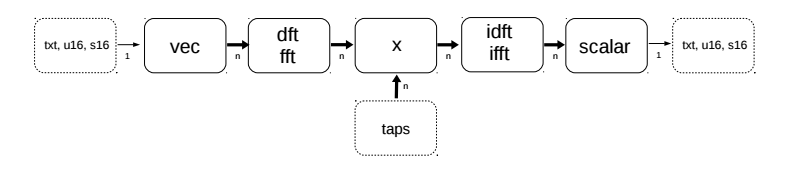
\includegraphics[width = 0.8 \textwidth]{flujo_senales}
		\caption{Flujo de procesamiento de señales.}
		\label{fig:flujo_senales}
	\end{figure}

	Como se ve en la Figura \ref{fig:flujo_senales}, a partir de una secuencia de números complejos entrantes, se los transforma (con vectorización previa), escala por el vector taps y luego anti-transforma saliendo como escalares.

	En principio, se utiliza como base la estructura del Trabajo Práctico 0, dado que éste también recibe parámetros por línea de órdenes y realiza operaciones con números complejos provistos por el flujo de entrada. En otras palabras, el diseño principal del presente trabajo se encuentra en la función de procesamiento \texttt{proc()} que engloba las operaciones representadas en la Figura \ref{fig:flujo_senales}.

	En primer lugar, suponiendo que se requiere poder utilizar el programa en tiempo real, se propone una iteración que procece de a bloques más pequeños la entrada, en vez de recibir la entrada completa y procesarla en su totalidad. Desde aquí se parte al primer bloque de procesamiento, que requiere almacenar la entrada en un vector de longitud dada por una variable de control. Para ello se hace uso de la biblioteca \texttt{<vector>}, la cual contiene una plantilla del tipo de dato vector. Dado que para el Trabajo Práctico 0 se tuvo que implementar la clase complejo, se reutilizó esa misma implementación en conjunto con el dato vector para modelar la entrada.

	Para el cálculo de transformaciones y anti-transformaciones se propone el uso de una clase abstracta \texttt{ft}. La clase abstracta (que no puede ser instanciada) tiene como fin darle abstracción a la implementación mientras se protegen los métodos de cálculo utilizados. Operativamente, se encarga de seleccionar que método de cómputo o síntesis utilizar (mediante las funciones \emph{getter's}) para que, al llamar a la función \texttt{calc()}, realice el cálculo requerido. En consecuencia, la función \texttt{proc()} llama a \texttt{calc()} que sobrescribe el vector entrante con su transformación.

	Entre transformaciones, se realiza el producto miembro a miembro entre coeficientes de transformación y ecualización (\texttt{taps}).

%%%%%%%%%%%%%%%%%%%%%%%%%%%%%%%%%%%%%%%%%%%% HASTA ACÁ HIZO %%%%%%%%%%%%%%%%%%%%%%%%%%%%%%%%%%%%%%%%%%%%%%%%%%%%%%%

%		En primer lugar se definió el algoritmo mediante el cual se realizaría el procesamiento de señales. 

%Se tuvo en cuenta el hecho de que, a partir del \textit{downsampling}, se desecha una cantidad importante de muestras. Específicamente, si se fijó un parámetro de decimación $N$, de cada $N$ muestras procesadas sólo una es finalmente utilizada. Por lo tanto sólo hace falta realizar los cálculos para las muestras que sabemos van a ``sobrevivir'' la decimación.

%Para cada muestra $n$, el \textit{moving average} realiza un promedio de las $N$ últimas muestras recibidas, es decir sigue la ecuación:

%	\begin{equation*}
%		 y[n] = \frac1N \sum_{k = 0}^{N-1} x[n-k]. 
%	\end{equation*}

%De lo anterior se sigue que cada muestra a la salida $y[n_0]$ es sólo función de los $N$ últimos valores a la entrada $x[n_0], x[n_0 - 1], \dots,  x[n_0 - N + 1]$. Los demás bloques de procesamiento sólo dependen del valor actual de su entrada, por lo que finalmente en el programa sólo hace falta recordar las últimas $N$ muestras que se recibieron para realizar los cálculos. 

%Con estas observaciones en mente, se optó por el siguiente algoritmo de implementación:

%	\begin{algorithmic}[H] % algorithmic fue el que pude hacer andar, porque me dejaba 
		       % redefinir las keywords. algorithm2e era mas lindo pero seteandolo
                       % con spanish y onelanguage mezclaba español con italiano.
		       % Si encontras uno que se vea mejor y en español es bienvenido.

		%\caption{Algoritmo para el procesamiento de las muestras.}
	
%		\While{el \textit{stream} de datos no termine}
%			\State $promedio := 0$
%			\For{las N siguientes muestras}
%				\State $promedio \gets promedio + x[n]$
%			\EndFor
%			\State $promedio \gets promedio / N$
%			\Return $\sqrt{\mathbf{Re}\{promedio\}^2 + \mathbf{Im}\{promedio\}^2}$ 
%		\EndWhile
%	\end{algorithmic}

\newpage

%%%%%%%%%%%%%%%%%%%%%%%%%%%%%%%%%%%%%%%%%%%%%%%%%%%%%%%%%%%%%%%%%%%%%

\subsection{Implementación}
 De acuerdo a lo requerido, la implementación de la herramienta se realizó en C++, para entradas y salidas de texto en los formatos especificados. Para ello se aprovecharon las clases \texttt{cmdline} y \texttt{complex} provistas en el curso, para el manejo de argumentos y números complejos respectivamente.

 Con respecto al manejo de argumentos, para utilizar la clase \texttt{cmdline} hace falta definir la tabla de opciones que se esperan recibir, de tipo \texttt{option\_t}. Se optó por definirla dentro del \texttt{main} del programa, con las siguientes opciones:

%	\lstinputlisting[firstline=48, lastline=54]{main.cc}

\lstset{language=C++}
\begin{lstlisting}[frame=single]
static option_t options[] = {
	{1, "i", "input", "-", opt_input, OPT_DEFAULT},
	{1, "o", "output", "-", opt_output, OPT_DEFAULT},
	{1, "N", "n_decimator","500",opt_n_decimator, OPT_DEFAULT},
	{0, "h", "help", NULL, opt_help, OPT_DEFAULT},
	{0, },
};
\end{lstlisting}

Como es requerido, se definió a la cadena ``-'' (tercera columna de la tabla de opciones) como el valor por defecto para las opciones de entrada y de salida. De esta manera, ya sea que se haya omitido esa opción o se la especifique explicítamente para que asuma su valor por defecto, en ambos casos se  obtendrá el mismo resultado.

Además la clase \texttt{cmdline} pide especificar las funciones que se utilizarán para \emph{parsear} cada opción (5ta columna de la tabla) - se las definió en el mismo \texttt{main}. Para las funciones que parsean las opciones de entrada, salida y ayuda se aprovecharon las que ya estaban implementadas en el archivo \texttt{main.cc} provisto con la implementación de la clase \texttt{cmdline} del curso. Quedó por definir, entonces, el \texttt{parser} para el parámetro $N$ de decimación:


\lstset{language=C++} 
\begin{lstlisting}[frame=single]
static void
opt_n_decimator(string const &arg)
{
	istringstream iss(arg);

	// Intentamos extraer el N de la linea de comandos.
	// Para detectar argumentos que unicamente consistan de
	// numeros enteros, vamos a verificar que EOF llegue justo
	// despues de la lectura exitosa del escalar
	
	if(!(iss >> n_decimator) || !iss.eof()) {
		cerr << "non-integer factor: "
		     << arg
		     << "."
		     << endl;
		exit(1);
	}

	if (iss.bad()) {
		cerr << "cannot read integer factor."
		     << endl;
		exit(1);
	}
}
\end{lstlisting}

Como el método \texttt{parse} de \texttt{cmdline} ya le pasa al \texttt{parser} su valor por defecto si fue omitido, siempre esta función recibirá un argumento para $N$ (no necesariamente válido). Se intenta leer el mismo como un entero, y de fallar se anuncia el error y se termina el programa. 

Los argumentos se leen mediante \texttt{cmdline.parse($\cdot$)} a cada una de las variables estáticas definidas fuera del \texttt{main}:

 
\lstset{language=C++}
\begin{lstlisting}[frame=single]
static size_t n_decimator;	// Decimator Factor (factor positivo de decimacion)
static istream *iss = 0;	// Input Stream (clase para manejo de los flujos de entrada)
static ostream *oss = 0;	// Output Stream (clase para manejo de los flujos de salida)
static fstream ifs; 		// Input File Stream (derivada de la clase ifstream que deriva de istream para el manejo de archivos)
static fstream ofs;		// Output File Stream (derivada de la clase ofstream que deriva de ostream para el manejo de archivos)
\end{lstlisting}

Estas son las variables que se le pasan a \texttt{am\_proc} que es la encargada de implementar el algoritmo de la sección anterior, de manera que el \texttt{main} queda:


\lstset{language=C++}
\begin{lstlisting}[frame=single]
int
main(int argc, char * const argv[])
{
	cmdline cmdl(options);	// Objeto con parametro tipo option_t (struct) declarado globalmente.
	cmdl.parse(argc, argv);	// Metodo de parseo de la clase cmdline
	am_proc(iss, oss, n_decimator);	// Procesamiento AM
}
\end{lstlisting}

La función \texttt{am\_proc} está declarada en ``\texttt{am\_proc.h}'' y definida en ``\texttt{am\_proc.cc}''. Fuera de comprobar si hubo errores de lectura, su implementación es en escencia el pseudo-código de la sección anterior:

\lstset{language=C++}
\begin{lstlisting}[frame=single]
void am_proc(istream *is, ostream *os, const size_t& n_decimator){
	
	bool eof_flag=false;
	size_t i;
	complejo c, aux; // c tendra la suma y aux sera el que recibe el complejo del stream	


	// Si entra un archivo vacio (primero lee EOF), corta el for y luego el while, devolviendo un vacio

	while(!eof_flag){
		
		// Se suman los primeros 'n_decimator' numeros hasta que corte 
		for(i=1; i<=n_decimator && ((*is)>>aux); i++)
			c += aux;
	
		// Compruebo si se llego a EOF
		if(is->eof())
			eof_flag=true;

		if(is->bad()){ 
		// El for termino por no poder guardar el caracter en x
			cerr	<< "Error: Cannot read complex on input stream"
				<< endl;
			exit(1);
		}		

		// Realizo el proemdio movil
		c=c / n_decimator;
			
		// Imprimo el valor absoluto
		*os << c.abs()<<endl;
	}
	
	if(os->bad()){
		cerr	<< "Error: Cannot write output file"
			<< endl;
		exit(1);
	}

}
\end{lstlisting}


%%%%%%%%%%%%%%%%%%%%%%%%%%%%%%%%%%%%%%%%%%%%%%%%%%%%%%%%%%%%%%%%%%%%%%%%

\subsection{Análisis de complejidad}

	En la presente sección se realiza el análisis de complejidad espacial y temporal de los algoritmos de transformación por definición (DFT/iDFT) y optimizada (FFT/iFFT).

	Para el análisis de complejidad temporal, se supone que la entrada tiene una longitud \emph{N}. En el caso del algoritmo de DFT/iDFT, se requiere recorrer la entrada en su totalidad (y realizar operaciones matemáticas de coste temporal asintótico \emph{O(1)}) para obtener un coeficiente de Fourier. Por lo tanto, el costo temporal de obtener un único coeficiente es \emph{O(N)}. En consecuencia, dado que la salida tendrá la misma longitud que la entrada, se deberán calcular \emph{N} coeficientes implicando $N \times N$ operaciones, resultando en una complejidad asintótica temporal $O(N^{2})$.\\
	En cuanto al análisis espacial, se deben considerar dos conjuntos de variables: las requeridas para el cálculo, y las resultantes del mismo. Suponiendo que el peor caso será aquel cuya entrada de tamaño \emph{N} sea muy grande, la salida resultante también tendrá tamaño \emph{N}($O(N)$) y será grande. Las variables de cálculo, sin embargo, ante cualquier valor \emph{N} entrante, se mantendrá siempre constante. Asintóticamente se puede decir que este conjunto de variables es de coste $O(1)$. Por medio de la regla de la suma\footnote{$f_1 \in O(g) \cap f_2 \in O(h) \implies f_1 + f_2 \in O(\max(g,h))$} se infiere que la complejidad espacial será $O(N)$.\\
	Como la iDFT difiere en dos operaciones matemáticas de la DFT (se conjuga el $W_N$ y se divide a la salida por la longitud), se aplica el mismo razonamiento obteniendo los mismos resultados.

	Al inspeccionar el algoritmo FFT, se observa la técnica recursiva de \emph{Dividir y Conquistar} al desglosar el problema en 2 sub-problemas (llamada recursiva), cada uno con la mitad de tamaño $\left(\frac{N}{2}\right)$. Luego la resolución de cada problema realiza operaciones de orden lineal recorriendo el vector proporcional al largo inicial $N$. Suponiendo que requiere un tiempo $T(N)$ de cómputo para una entrada de longitud $N$, la ecuación en recurrencia queda determinada como:

		\begin{equation*}
			T(N) = 2 \cdot T\left(\frac{N}{2}\right) + O(N)
		\end{equation*}
	Dado que la ecuación sigue la forma:

		\begin{equation*}
			T(N) = a \cdot T\left(\frac{N}{b}\right) + f(N)
		\end{equation*}
	y se cumple que $a=2\geq1$ y $b=2\geq1$, se puede aplicar el teorema maestro concluyendo que, como $a=b^1$, $T(N)\in \Theta(N^1 \cdot \log(N))$. Por lo tanto, la complejidad temporal asintótica es $\Theta(N\cdot \log(N))$.
	Si se analiza el coste espacial, se debe considerar que, al hacer la llamada recursiva, se generan dos vectores de tamaño $\frac{N}{2}$. En otras palabras, se requiere de memoria de tamaño $N$. La recursión seguirá hasta el punto de pedir memoria de tamaño 1, pero N veces. En consecuencia, se requiere \emph{N} veces de bloques de tamaño \emph{N} de memoria. Por lo tanto, el coste espacial es asintóticamente $O(N^2)$.
	Al igual que con la DFT y la iDFT, existe la dualidad de la FFT con la iFFT, validando el desarrollo previo para la anti-transformada.	


	\section{Proceso de compilación} 	\label{sec:comp}
		
Para el manejo del proyecto se optó por utilizar la herramienta \texttt{make} por sobre la compilación manual, dado que \texttt{make} evalua si los archivos fuente fueron modificados después de la compilación y sólo ejecuta los scripts necesarios. Además mantiene al proyecto ordenado y facilita su desarrollo. A continuación se presenta el archivo \texttt{Makefile} que se encuentra en el directorio que contiene todos los archivos fuente y se ejecuta desde la terminal de UNIX simplemente insertando el comando \texttt{make} o en su defecto \texttt{make all}. 

	\lstinputlisting[language=make]{Makefile}



	\section{Corridas de prueba}
		
Para realizar las corridas de prueba del trabajo, se implementó una serie de scripts que se ejecutan en conjunto bajo el comando \texttt{make test} \footnote{Dicho comando llama en primer instancia al target \texttt{tp1.exe}, en caso de que no se haya compilado el programa previamente}. A continuación se describen cada uno de ellos:

	\begin{itemize}
		\item \textbf{Test 1}. Comprueba si ante una entrada vacía, se genera una salida vacia.
		\item \textbf{Test 2}. Si la entrada tiene menos de $n$ elementos, donde $n$ es la longitud del vector de muestras, debe completarse con ceros. Paraprobar esto, suponiendo que las operaciones de transformación y anti-transformación son correctas, con una entrada de las condiciones expresadas anteriormente la salida debe ser igual con la excepción de los valores nulos restantes.
		\item \textbf{Test 3}. Se prueba si el programa tiene la capacidad de procesar números reales a la entrada.
		\item \textbf{Test 4}. Idem pero ante entradas del tipo complejas.
		\item \textbf{Test 5}. Este \emph{test} se encarga de verificar si los cálculos de transformadas y anti-transformadas son correctos. Ésto se comprueba comparando la similitud entre la entrada y la salida.
		\item \textbf{Test 6}. Valida si la implementación de la ecualización es correcta.
	\end{itemize}

Cabe destacar el hecho de que no se comprueba el funcionamiento de la interpretación de la línea de comandos dado que esa validación tuvo lugar en el trabajo práctico pasado.


	
	\section{Código fuente}
		
A continuación se presentan los códigos fuente que forman parte del proyecto:

	\lstinputlisting{main.cc}
	\lstinputlisting{cmdline.h}
	\lstinputlisting{cmdline.cc}
	\lstinputlisting{complejo.h}
	\lstinputlisting{complejo.cc}
	\lstinputlisting{ft.h}
	\lstinputlisting{ft.cc}
	\lstinputlisting{proc.h}
	\lstinputlisting{proc.cc}



\end{document}
